%%%%%%%%%%%%%%%%%%%%%%%%%%%%%%%%%%%%%%%%%%%%%%%%%%%%%%%%%%%%%%%%%%%%%%%%%%%
%
% Template for a LaTex article in English.
%
%%%%%%%%%%%%%%%%%%%%%%%%%%%%%%%%%%%%%%%%%%%%%%%%%%%%%%%%%%%%%%%%%%%%%%%%%%%

\documentclass{article}

% AMS packages:
\usepackage{amsmath, amsthm, amsfonts}
\usepackage[utf8]{inputenc}
\usepackage[T1]{fontenc}
\usepackage[colorlinks=true,breaklinks=true,linkcolor=blue]{hyperref}
\usepackage[french]{babel}
\usepackage{graphicx}
\usepackage{pdfpages}

% Theorems
%-----------------------------------------------------------------
\newtheorem{thm}{Theorem}[section]
\newtheorem{cor}[thm]{Corollary}
\newtheorem{lem}[thm]{Lemma}
\newtheorem{prop}[thm]{Proposition}
\theoremstyle{definition}
\newtheorem{defn}[thm]{Definition}
\theoremstyle{remark}
\newtheorem{rem}[thm]{Remark}

% Shortcuts.
% One can define new commands to shorten frequently used
% constructions. As an example, this defines the R and Z used
% for the real and integer numbers.
%-----------------------------------------------------------------
\def\RR{\mathbb{R}}
\def\ZZ{\mathbb{Z}}

% Similarly, one can define commands that take arguments. In this
% example we define a command for the absolute value.
% -----------------------------------------------------------------
\newcommand{\abs}[1]{\left\vert#1\right\vert}

\renewcommand{\thesection}{\arabic{section} -}
%\renewcommand{\thesection}{\Roman{section}}
%\renewcommand{\thesection}{\Alph{section}}

%%%% Pour réaliser un Tableau %%%%
\usepackage{array,multirow,makecell}
\setcellgapes{1pt}
\makegapedcells
\newcolumntype{R}[1]{>{\raggedleft\arraybackslash }b{#1}}
\newcolumntype{L}[1]{>{\raggedright\arraybackslash }b{#1}}
\newcolumntype{C}[1]{>{\centering\arraybackslash }b{#1}}

% Operators
% New operators must defined as such to have them typeset
% correctly. As an example we define the Jacobian:
% -----------------------------------------------------------------
\DeclareMathOperator{\Jac}{Jac}

%-----------------------------------------------------------------
\title{Audit}
\author{Samir Mehal\\
  \small ToDo \& Co\\
  \small Openclassrooms - Projet 8\\
  \small France
}

\begin{document}
\maketitle

%\abstract{}

\newpage

\tableofcontents

\newpage

%\section*{Introduction}
%\addcontentsline{toc}{section}{Introduction}



\section{Résumé du projet}

Le projet ToDo \& Co est un site web qui permet de créer et de modifier des utilisateurs ainsi que de créer et de modifier des tâches. Le but de ce document est de réaliser un audit du site web tel qu'il est ainsi qu'un audit du site web après ajout des modifications demandées ainsi que des tests. Le site web a été refait from scratch car les versions de PHP et de Symfony utilisées étaient trop anciennes. Nous sommes passés de la version 5.5.9 de PHP à la version 8.2, et de la version 3.1 de Symfony à la version 7.0.

\section{Audit}

Un audit d'un site web est une analyse de la qualité de son code et de ses performances. Pour auditer la qualité du code, nous utiliserons Codacy de Symfony et pour auditer la performance nous utiliserons le profiler de Symfony.

\subsection{Codacy}

Codacy automatise les révisions de code et surveille la qualité du code à chaque demande de validation et d'extraction. Il rapporte l'impact de chaque demande de validation ou d'extraction sur les nouveaux problèmes concernant le style de code, les meilleures pratiques, la sécurité et bien d'autres.

Codacy s'utilise sur le repository de Github, ici sur le projet ToDo \& Co.

\subsubsection{Projet avec Symfony 3}

En utilisant Codacy sur le repository du projet avec Symfony 3, nous obtenons le résultat suivant : 

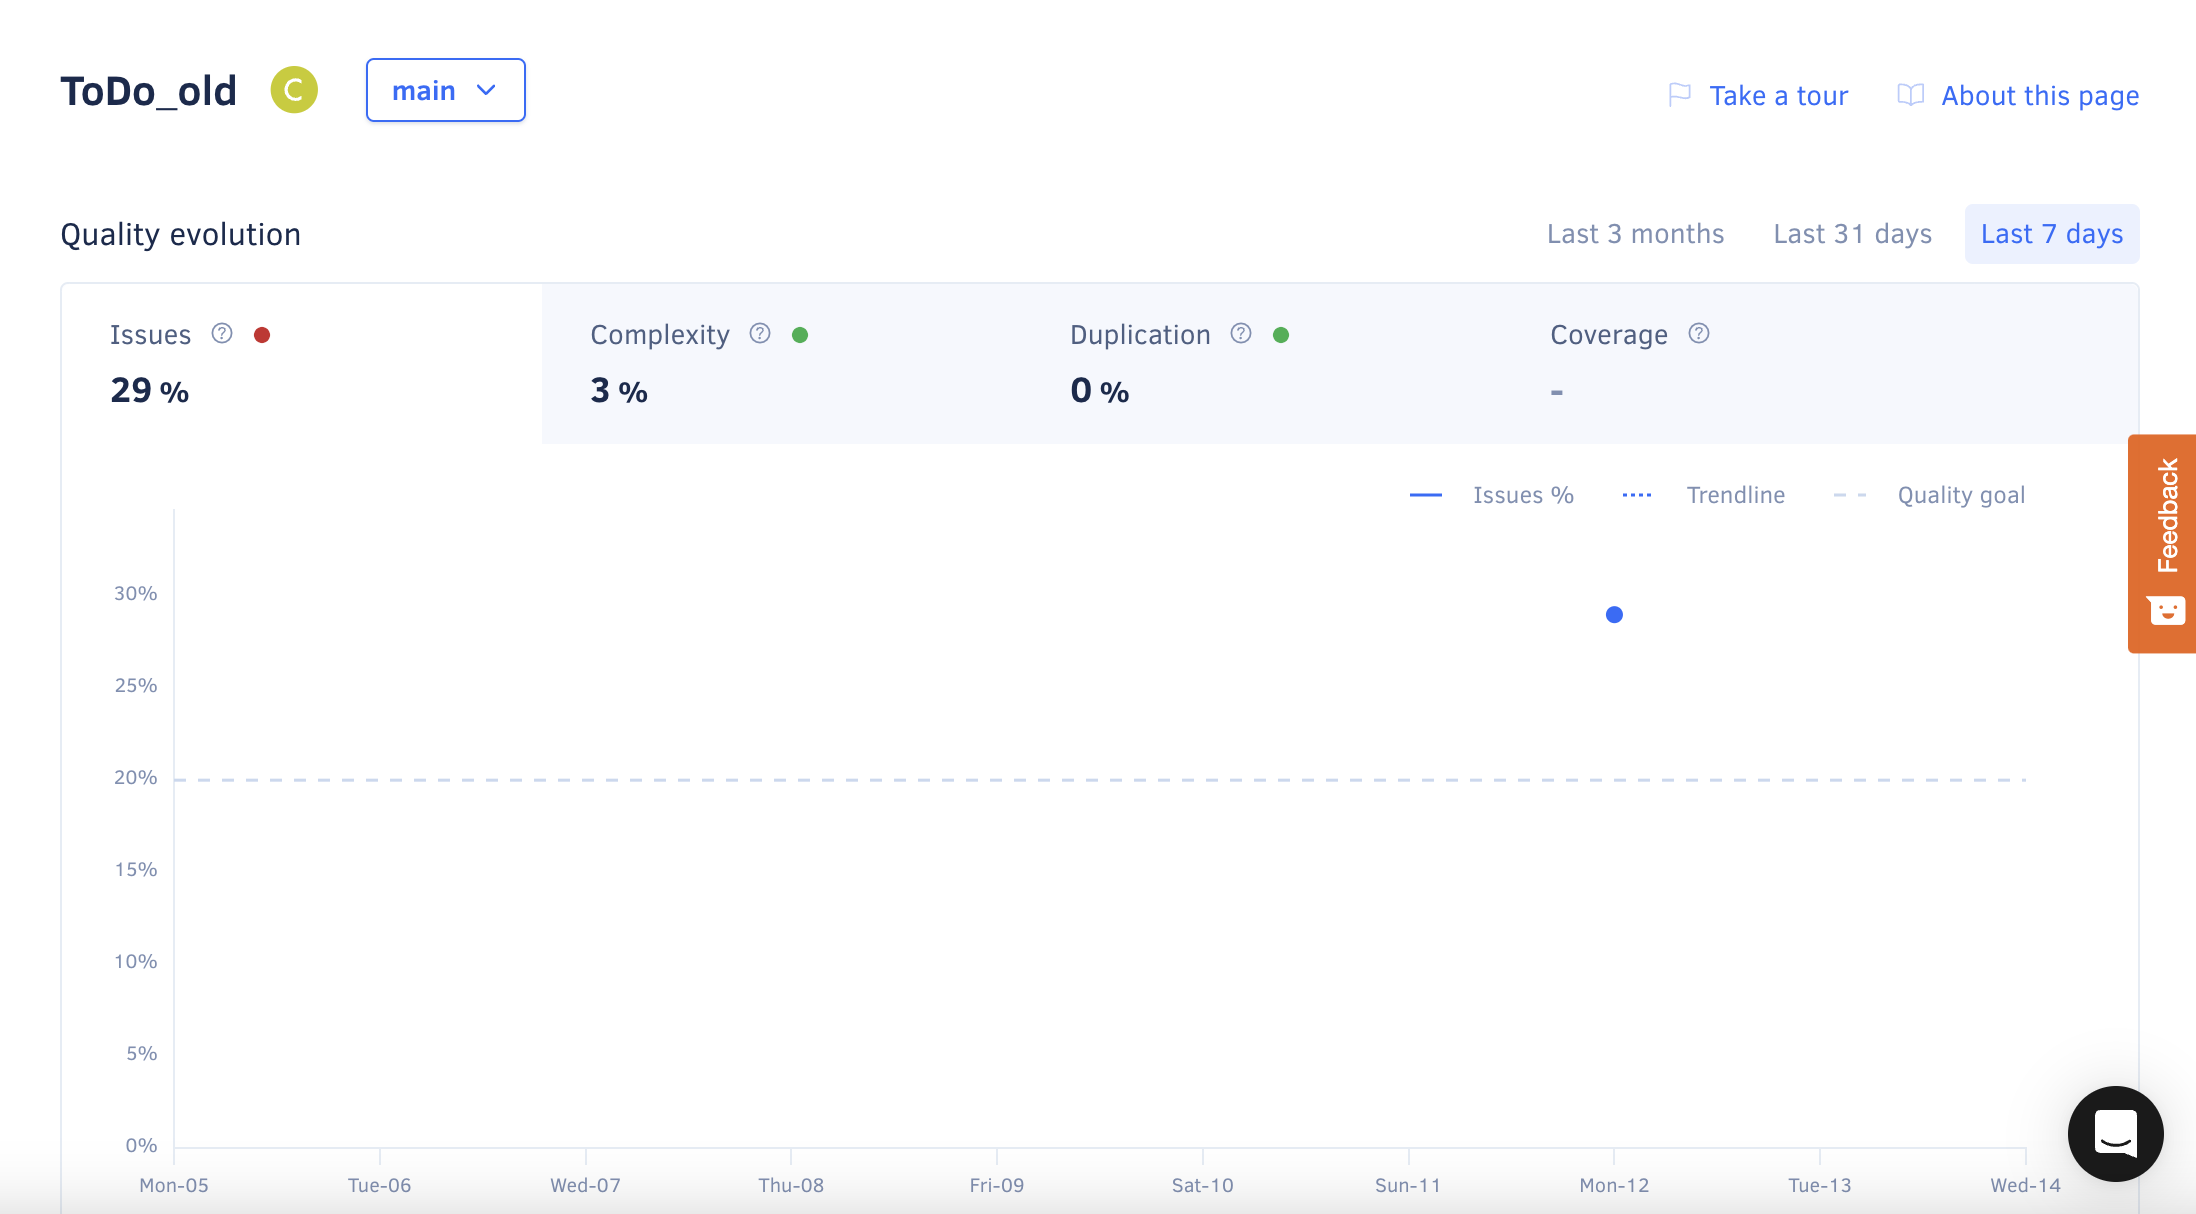
\includegraphics[scale=0.4]{Capture_ToDo_old/ToDo_old_1.png}

\hspace*{2cm}

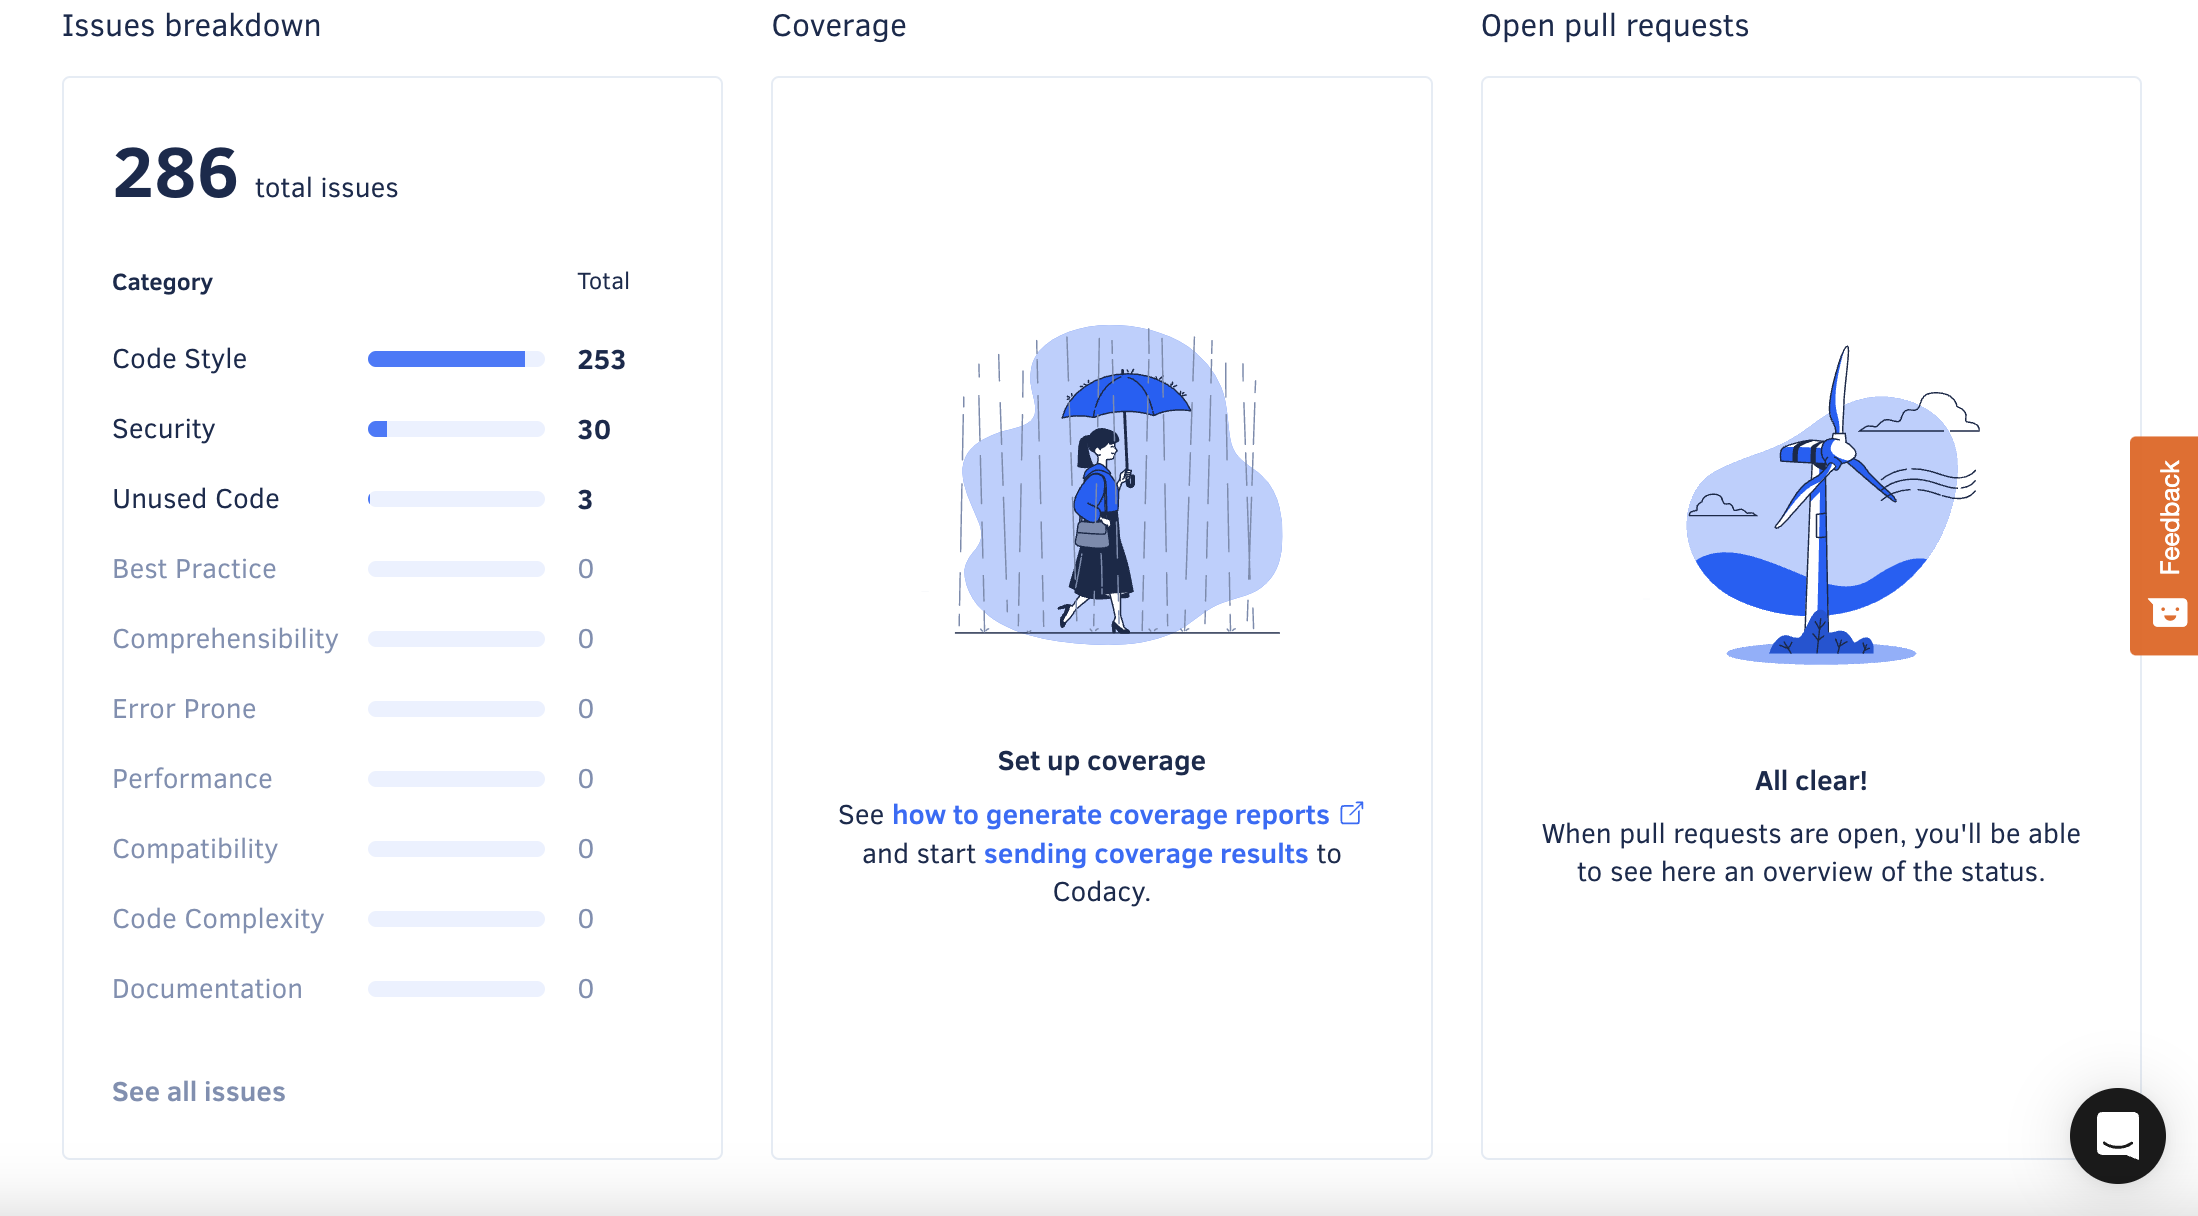
\includegraphics[scale=0.4]{Capture_ToDo_old/ToDo_old_2.png}

\subsubsection{Projet avec Symfony 7 avant modification}

En utilisant Codacy sur le repository du projet avec Symfony 7 avant d'ajouter les modifications, nous obtenons le résultat suivant : 

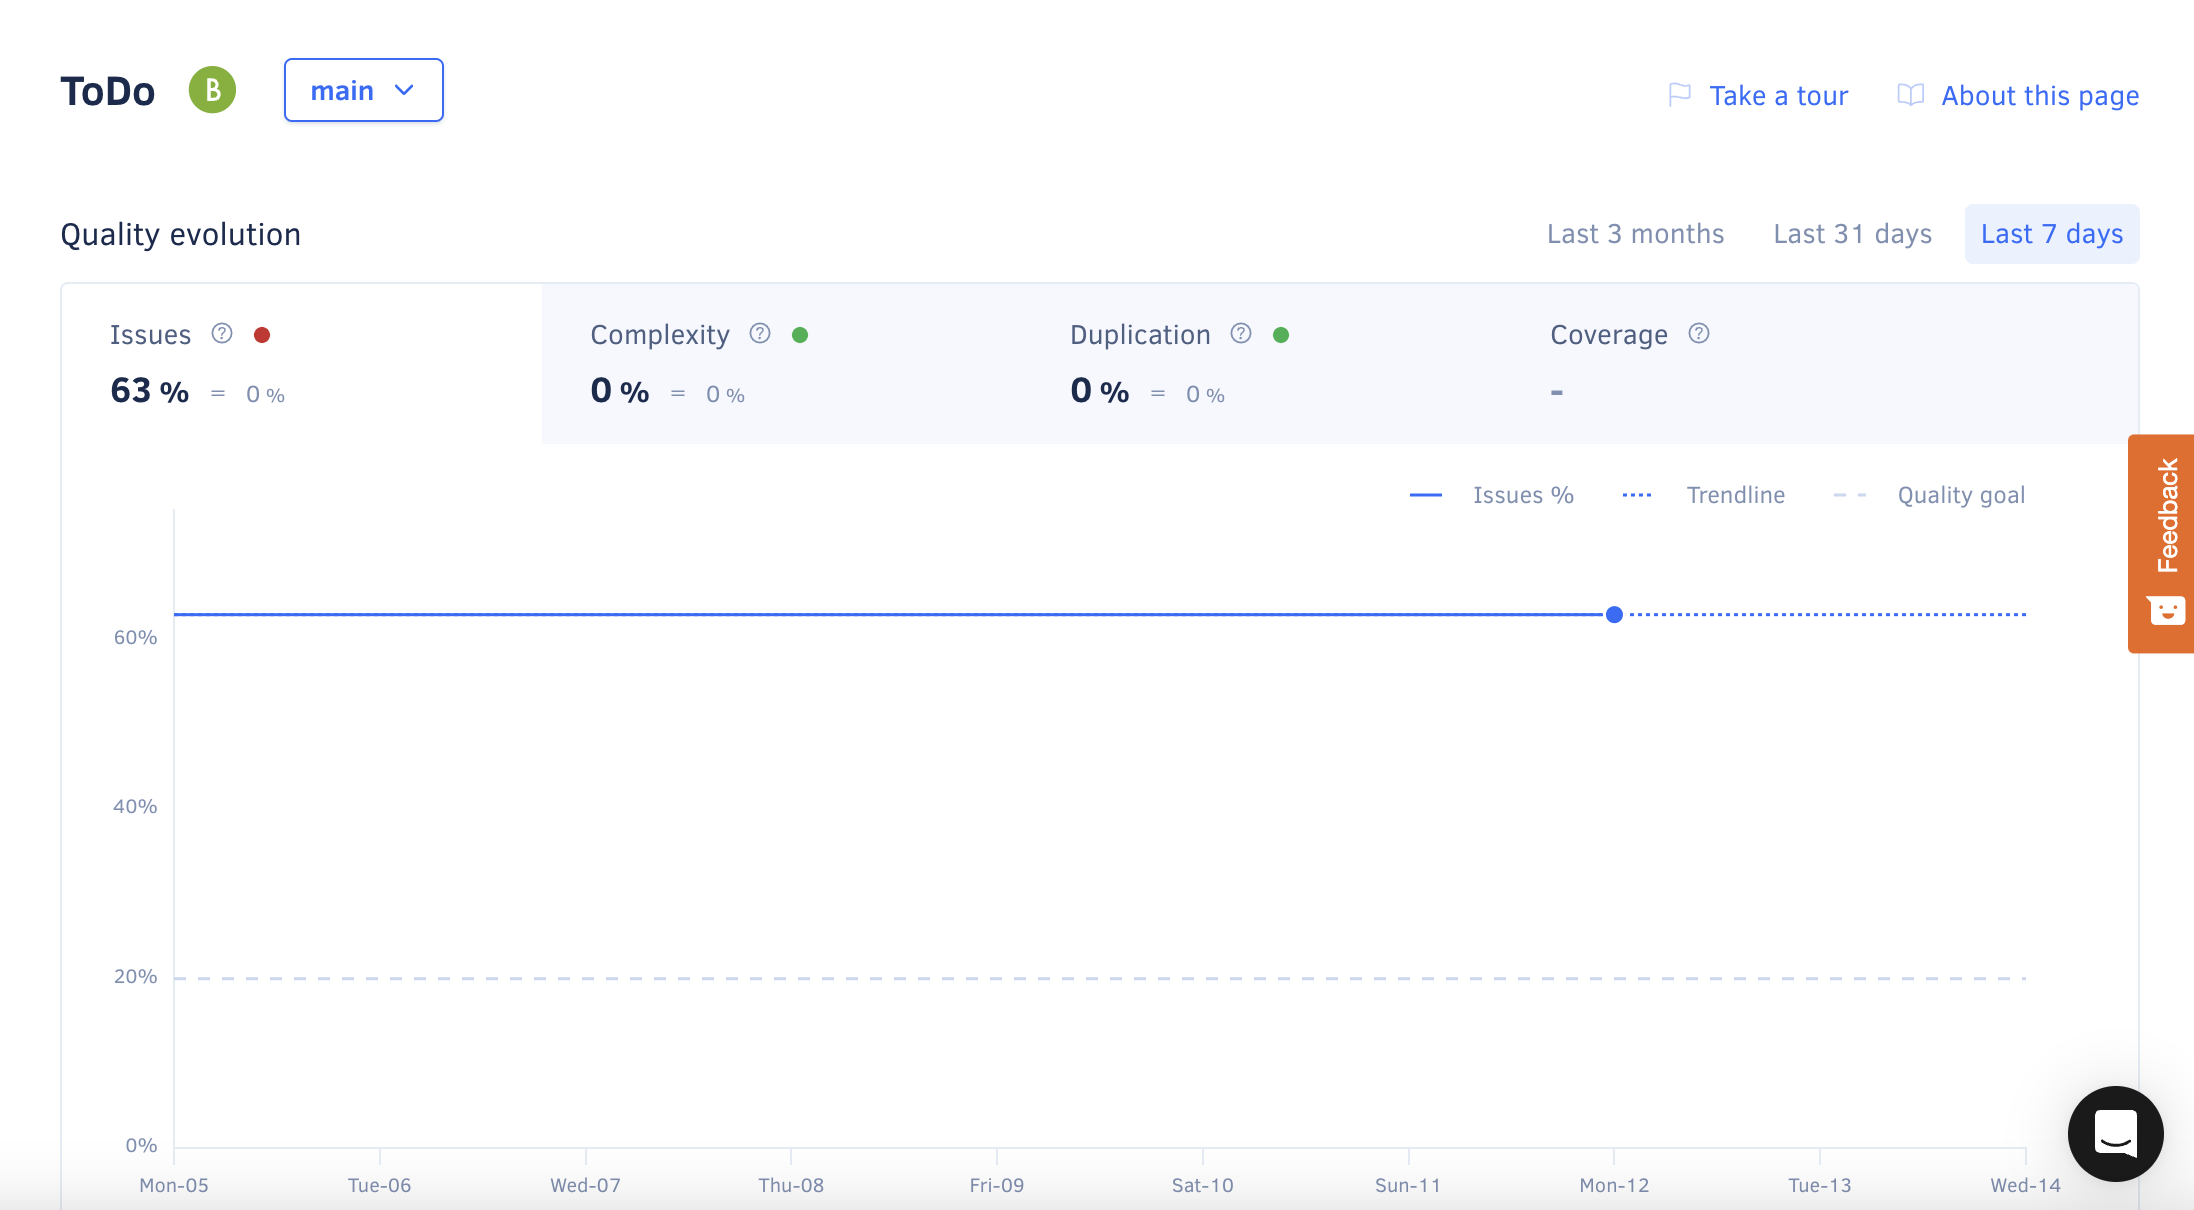
\includegraphics[scale=0.4]{Capture_new_avant_modif/ToDo_new_avant_modif_1.png}

\hspace*{2cm}

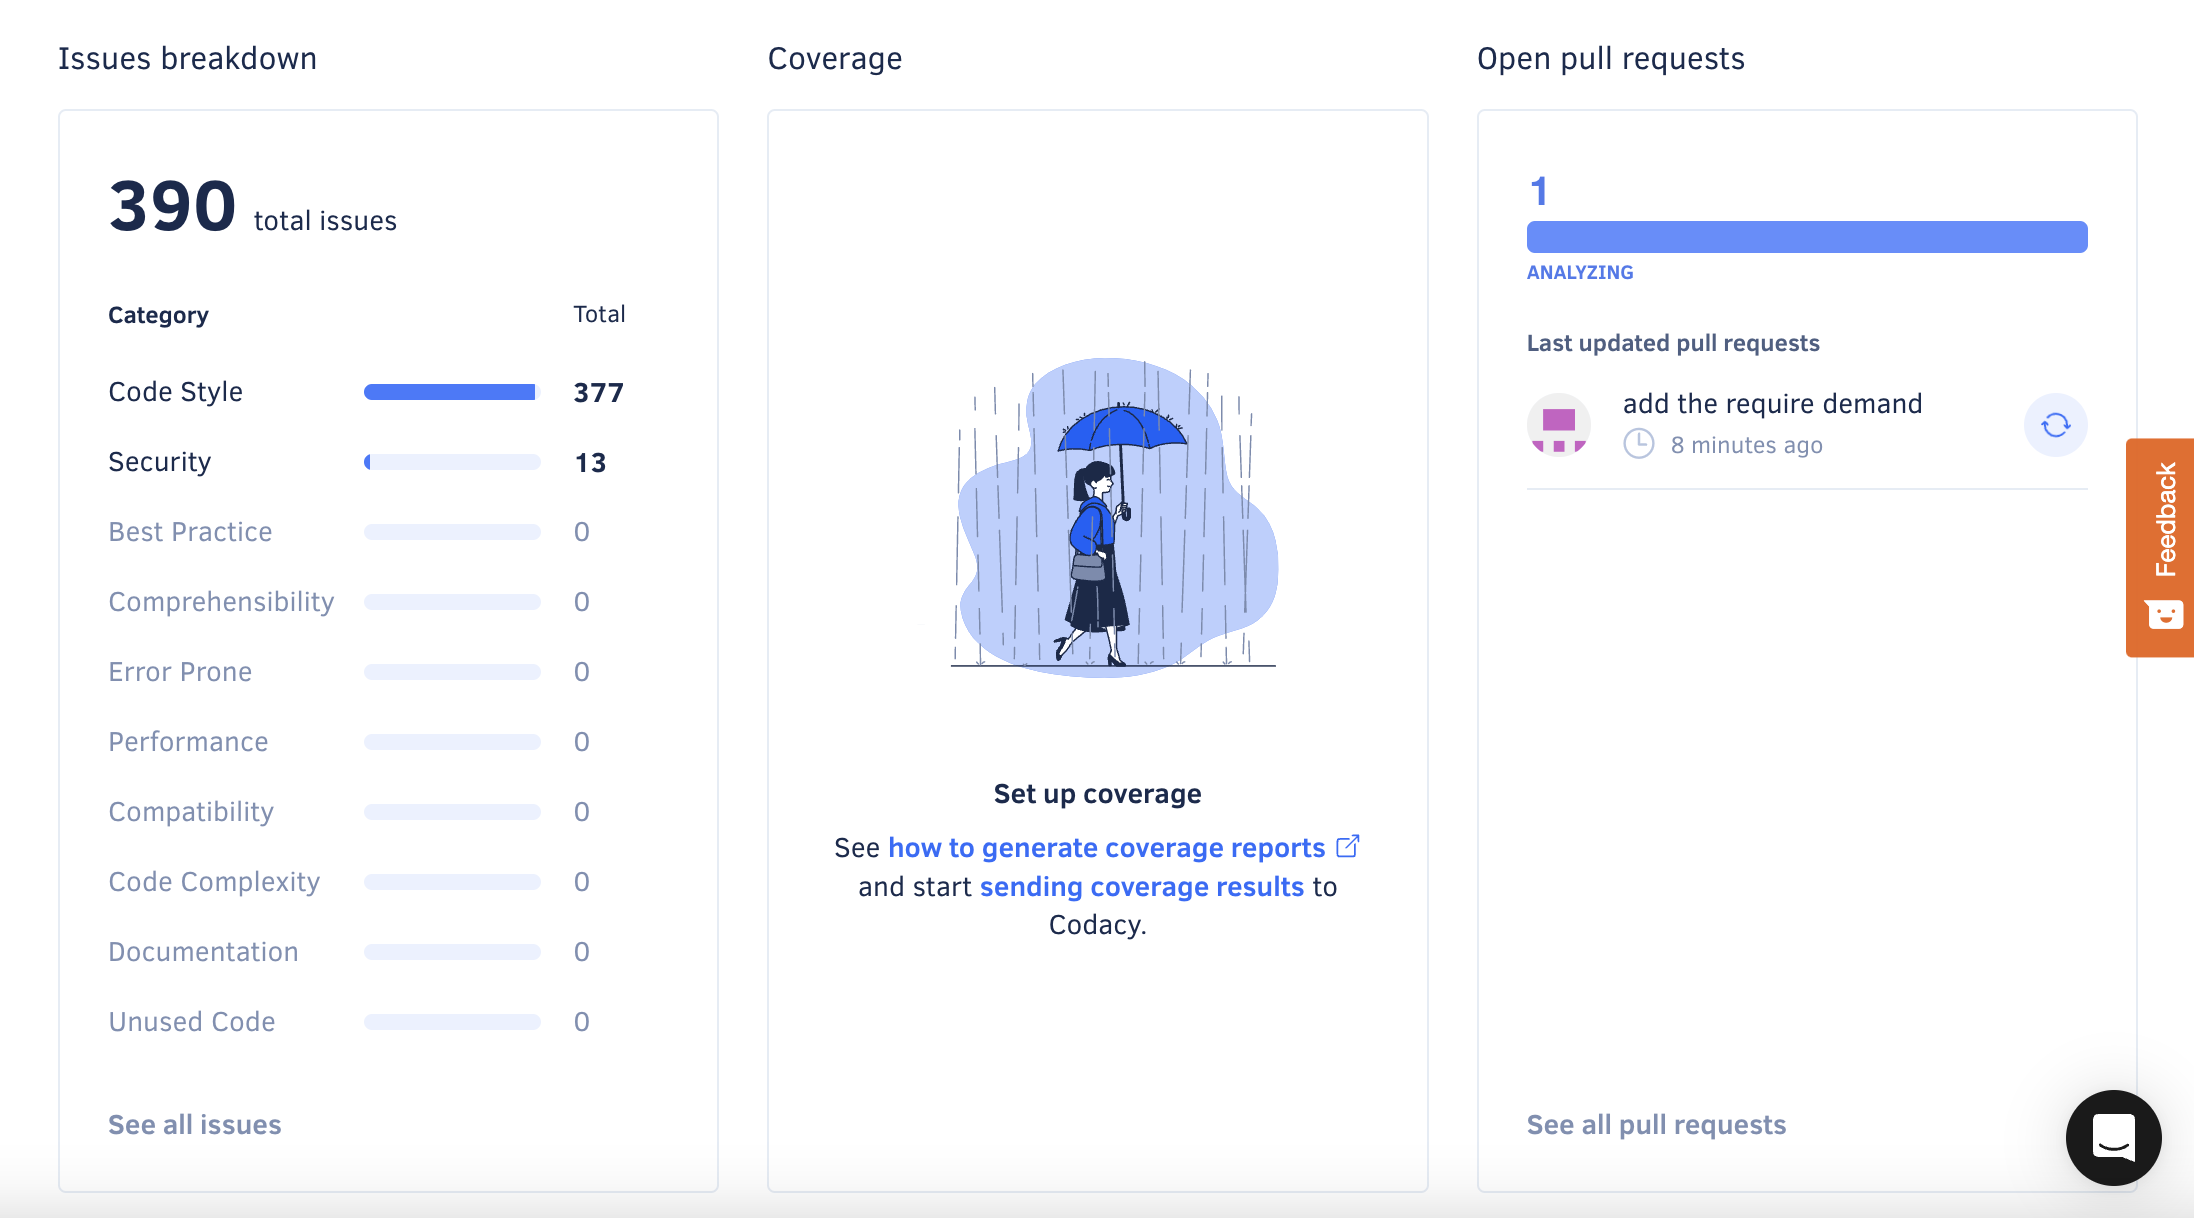
\includegraphics[scale=0.4]{Capture_new_avant_modif/ToDo_new_avant_modif_2.png}

\subsubsection{Projet avec Symfony 7 après modification}

En utilisant Codacy sur le repository du projet avec Symfony 7 après avoir ajouter les modifications et écrit les tests unitaires et fonctionnels, nous obtenons le résultat suivant : 

\hspace*{2cm}

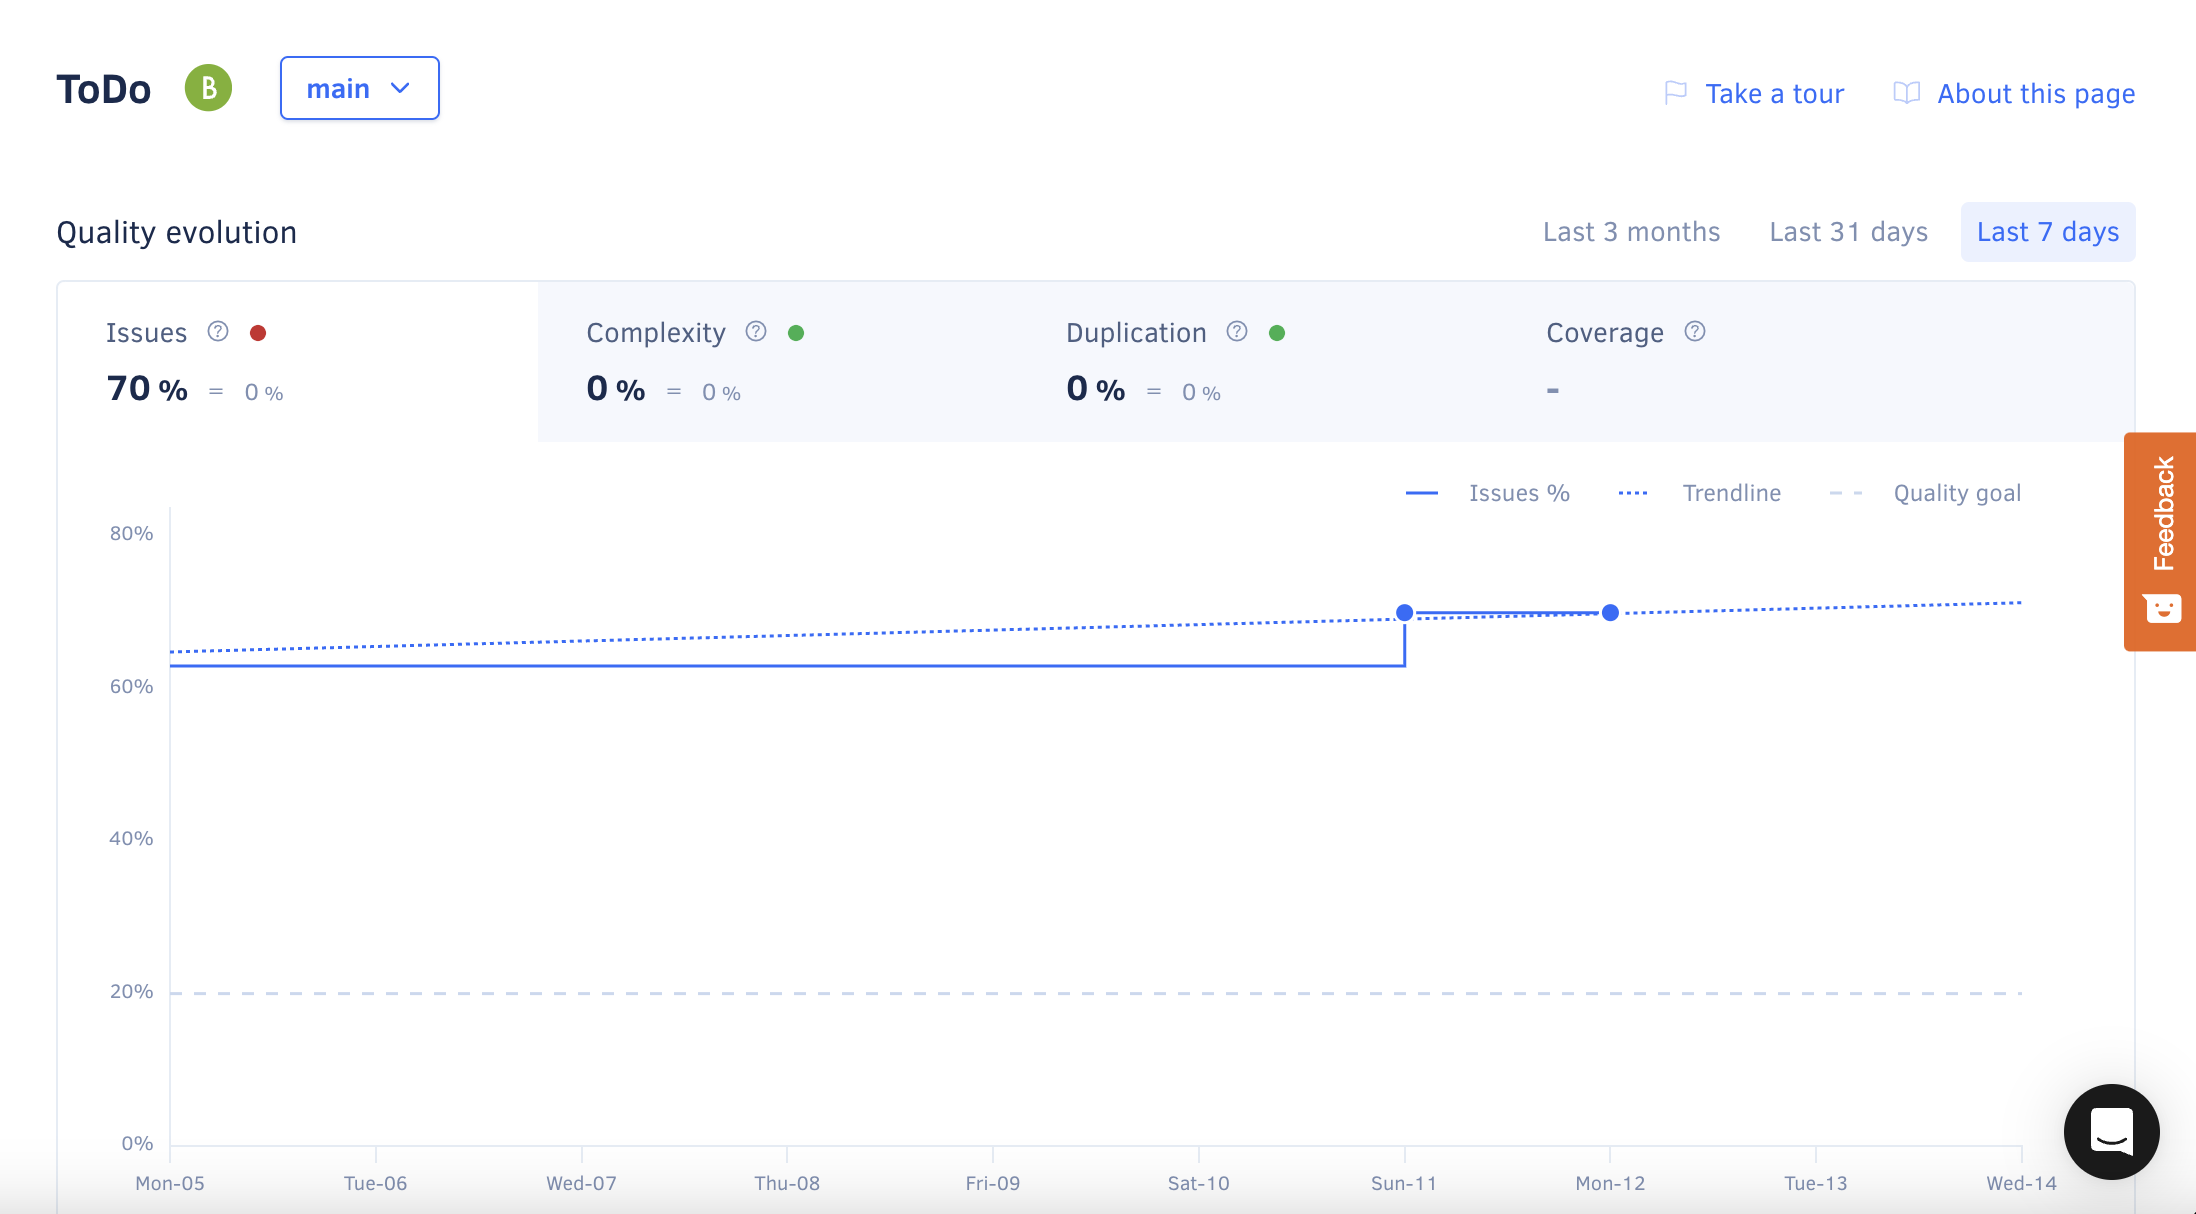
\includegraphics[scale=0.4]{Capture_ToDo/ToDo_new_1.png}

\hspace*{2cm}

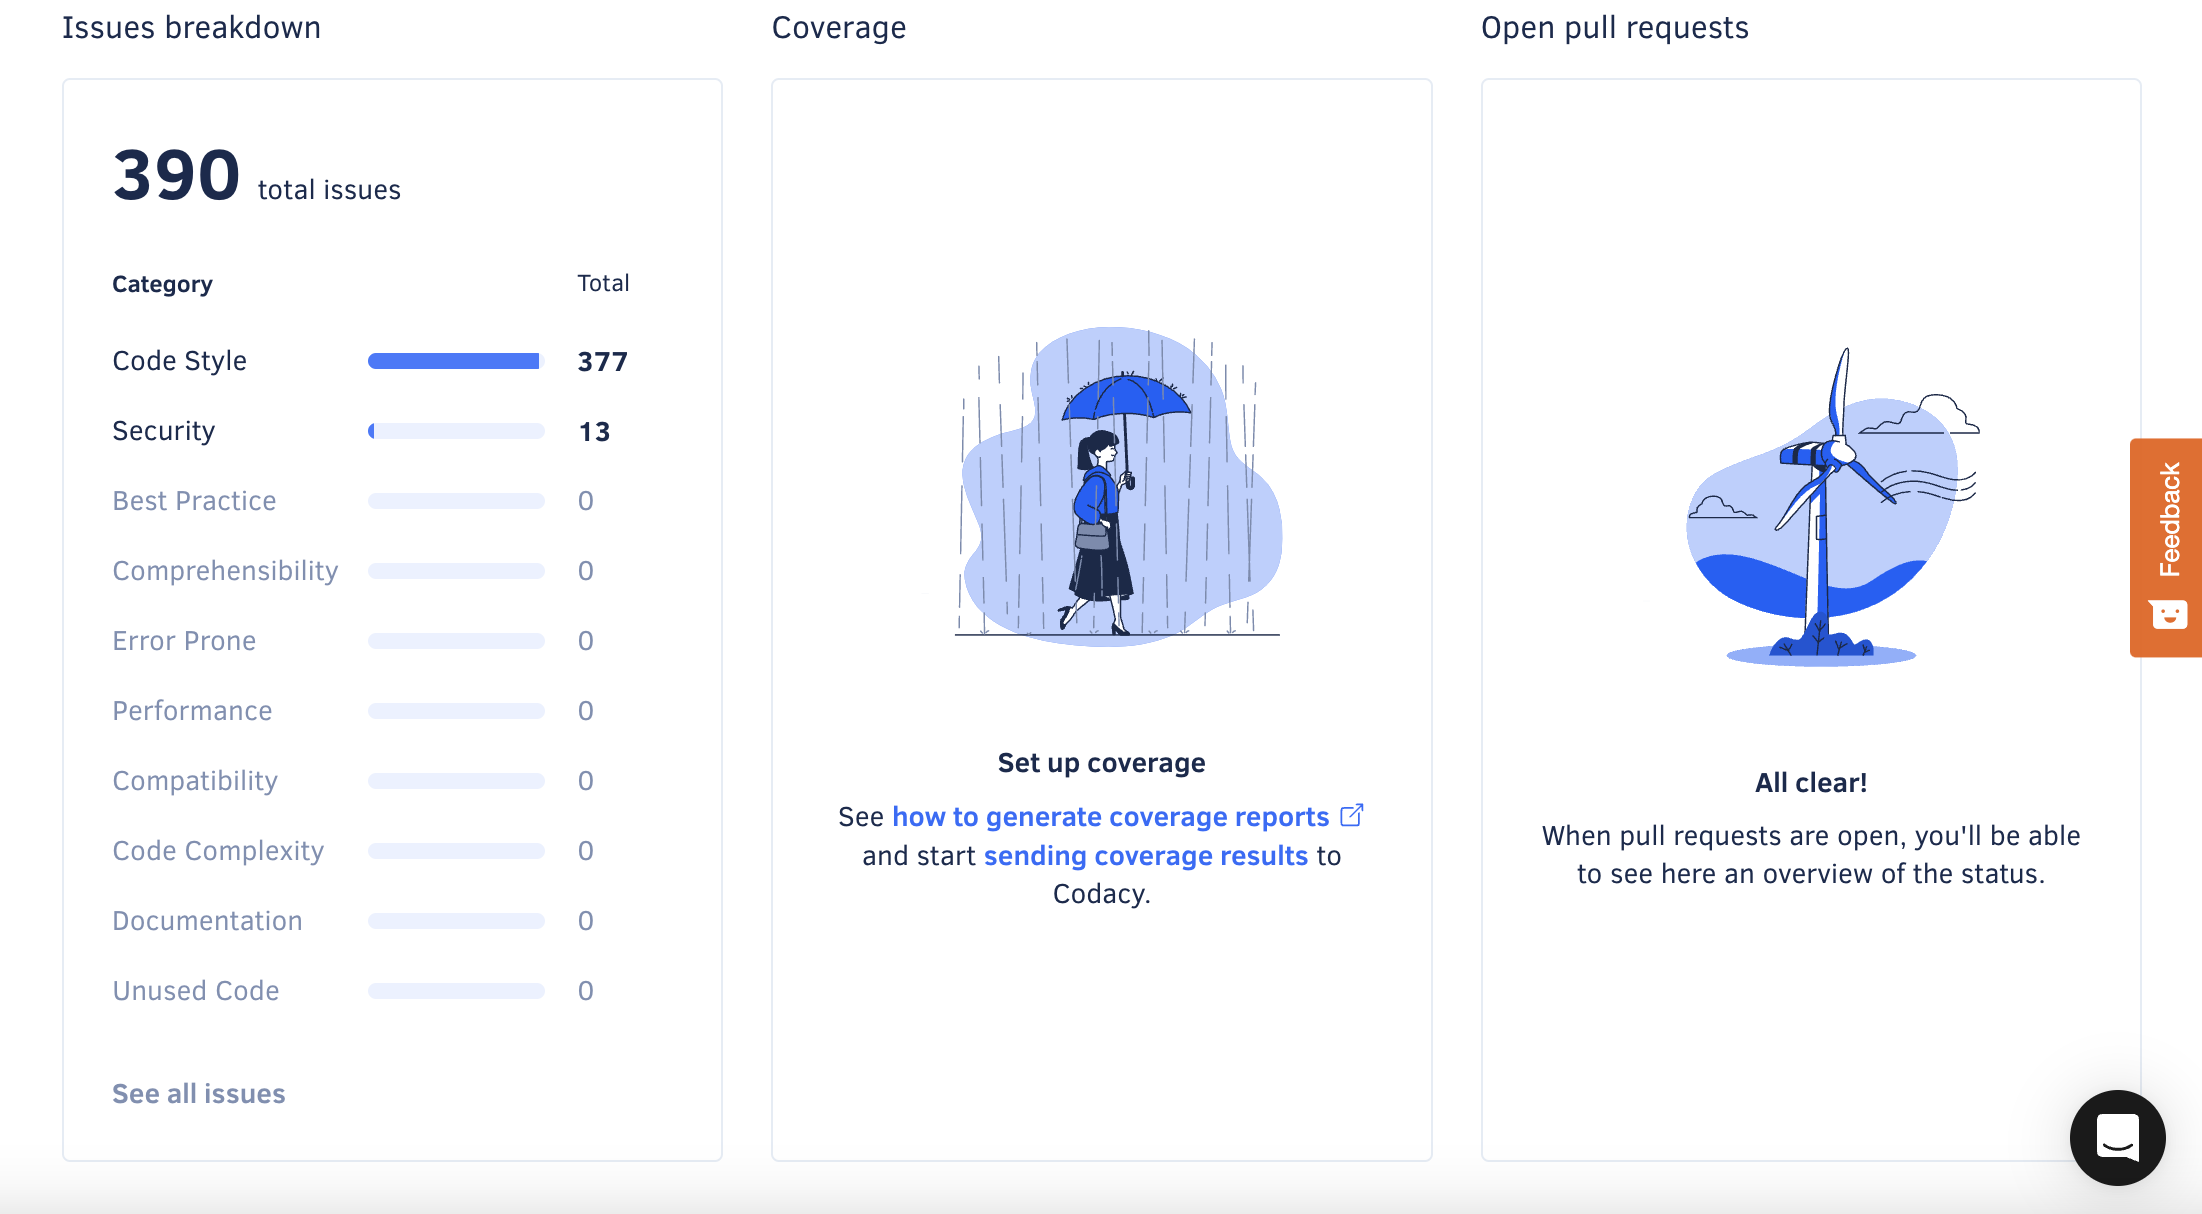
\includegraphics[scale=0.4]{Capture_ToDo/ToDo_new_2.png}

\subsubsection{Comparaison}

Plus le projet est récent et plus il possède de modifications, ce qui explique que le pourcentage d'issues augmente. Le nombre d'issue augmente aussi mais dans le projet avec Symfony 7 et après modification, des fichiers correspondant aux fichiers internent à Symfony ont été ignoré pour améliorer l'analyse de Codacy et donc la note globale. Le projet reste globalement le même, seul deux trois ajouts ont été réalisés (ajout d'un auteur aux tâches, seul ceux qui ont créé une tâche peuvent la supprimer, seul les administrateur peuvent accéder aux pages utilisateurs et choix du rôle lors de la création et de la modification d'un utilisateur).

\subsection{Profiler de Symfony}

Le Web Profiler est une application Symfony livrée avec le framework Standard Edition et disponible quand nous travaillons en environnement de développement. Il permet de collecter de nombreuses informations sur notre application durant son exécution comme le temps de rendu de la page, la consommation de mémoire, le nombre d'appels au cache, etc.

\subsubsection{Projet avec Symfony 7 avant modification}

En utilisant le Profiler de Symfony sur le repository du projet avec Symfony 7 avant d'ajouter les modifications, nous obtenons le résultat suivant : 


\includegraphics[scale=0.4]{Capture_profiler_avant_modif/Profiler_old_homepage.png}

\hspace*{2cm}

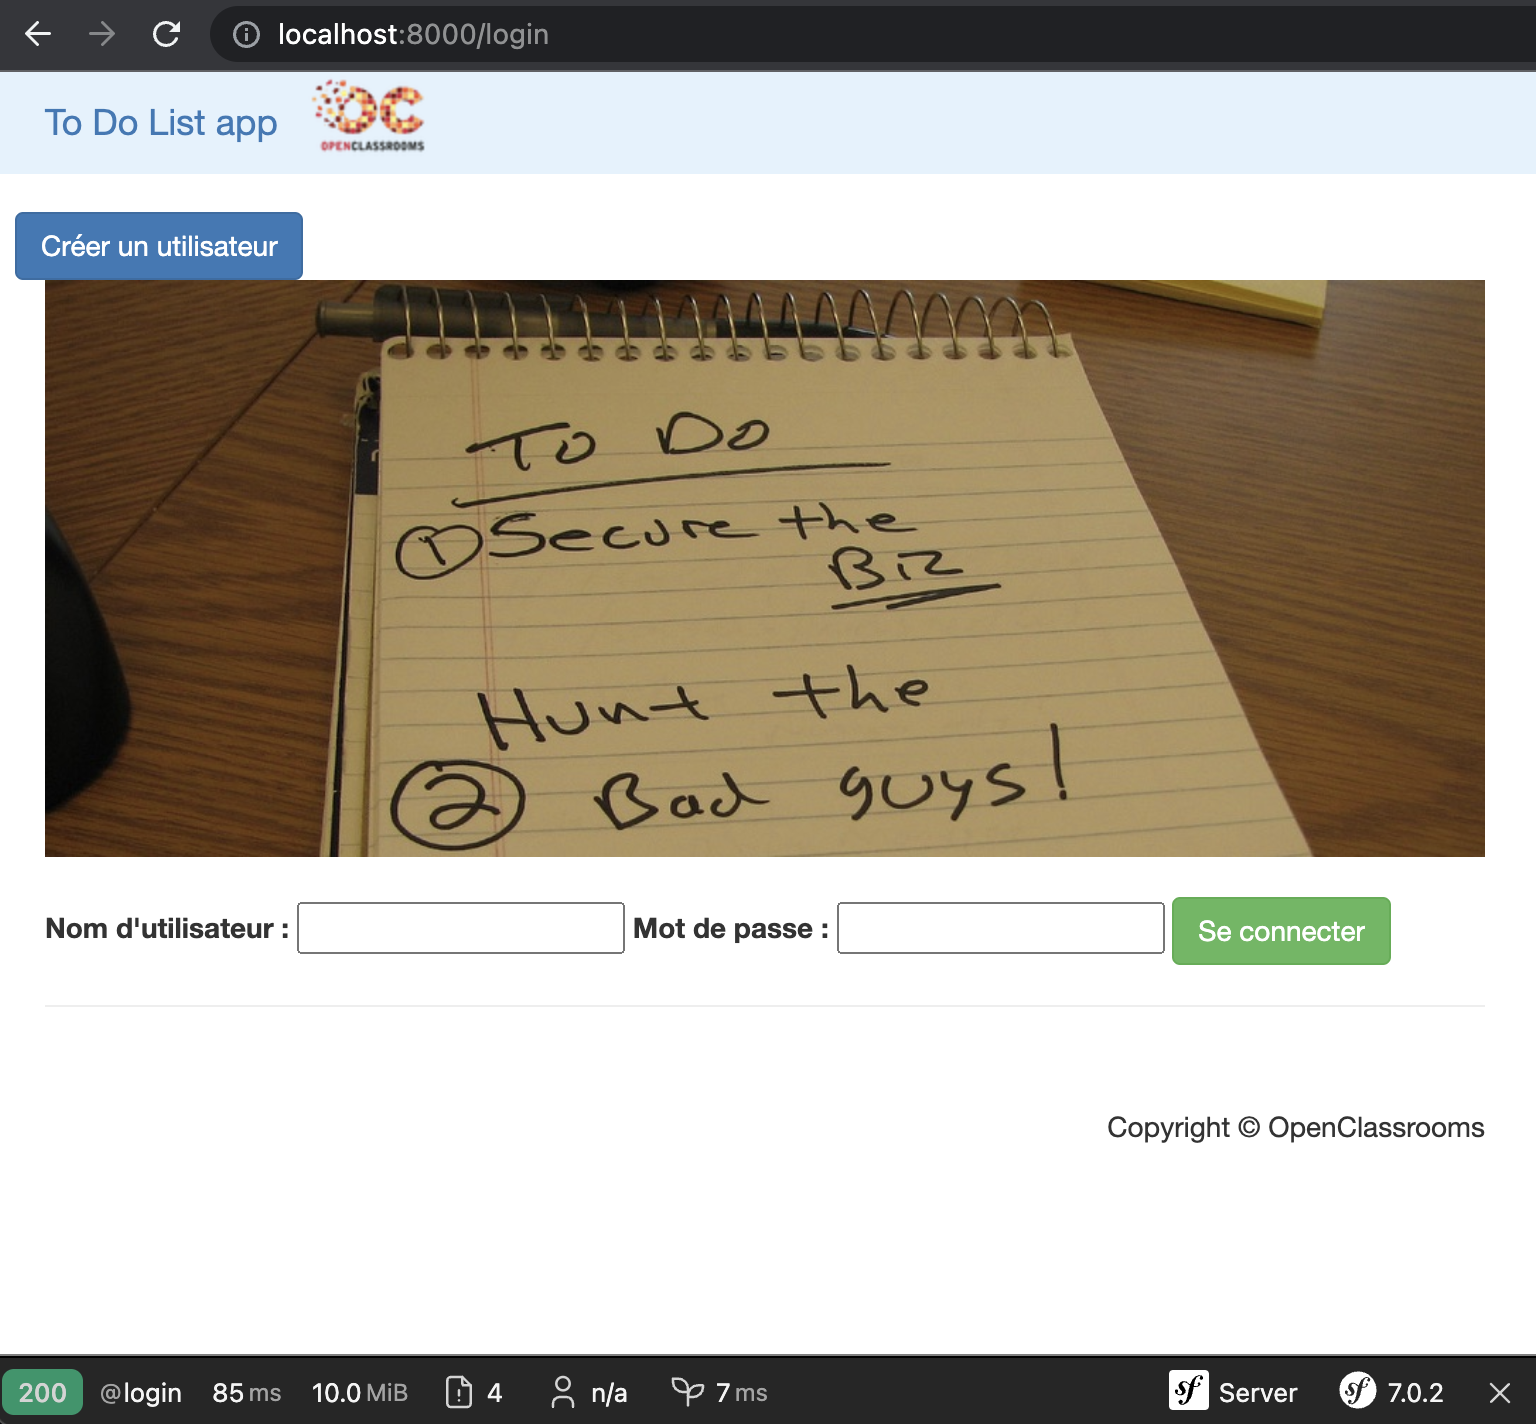
\includegraphics[scale=0.4]{Capture_profiler_avant_modif/Profiler_old_login.png}

\hspace*{2cm}

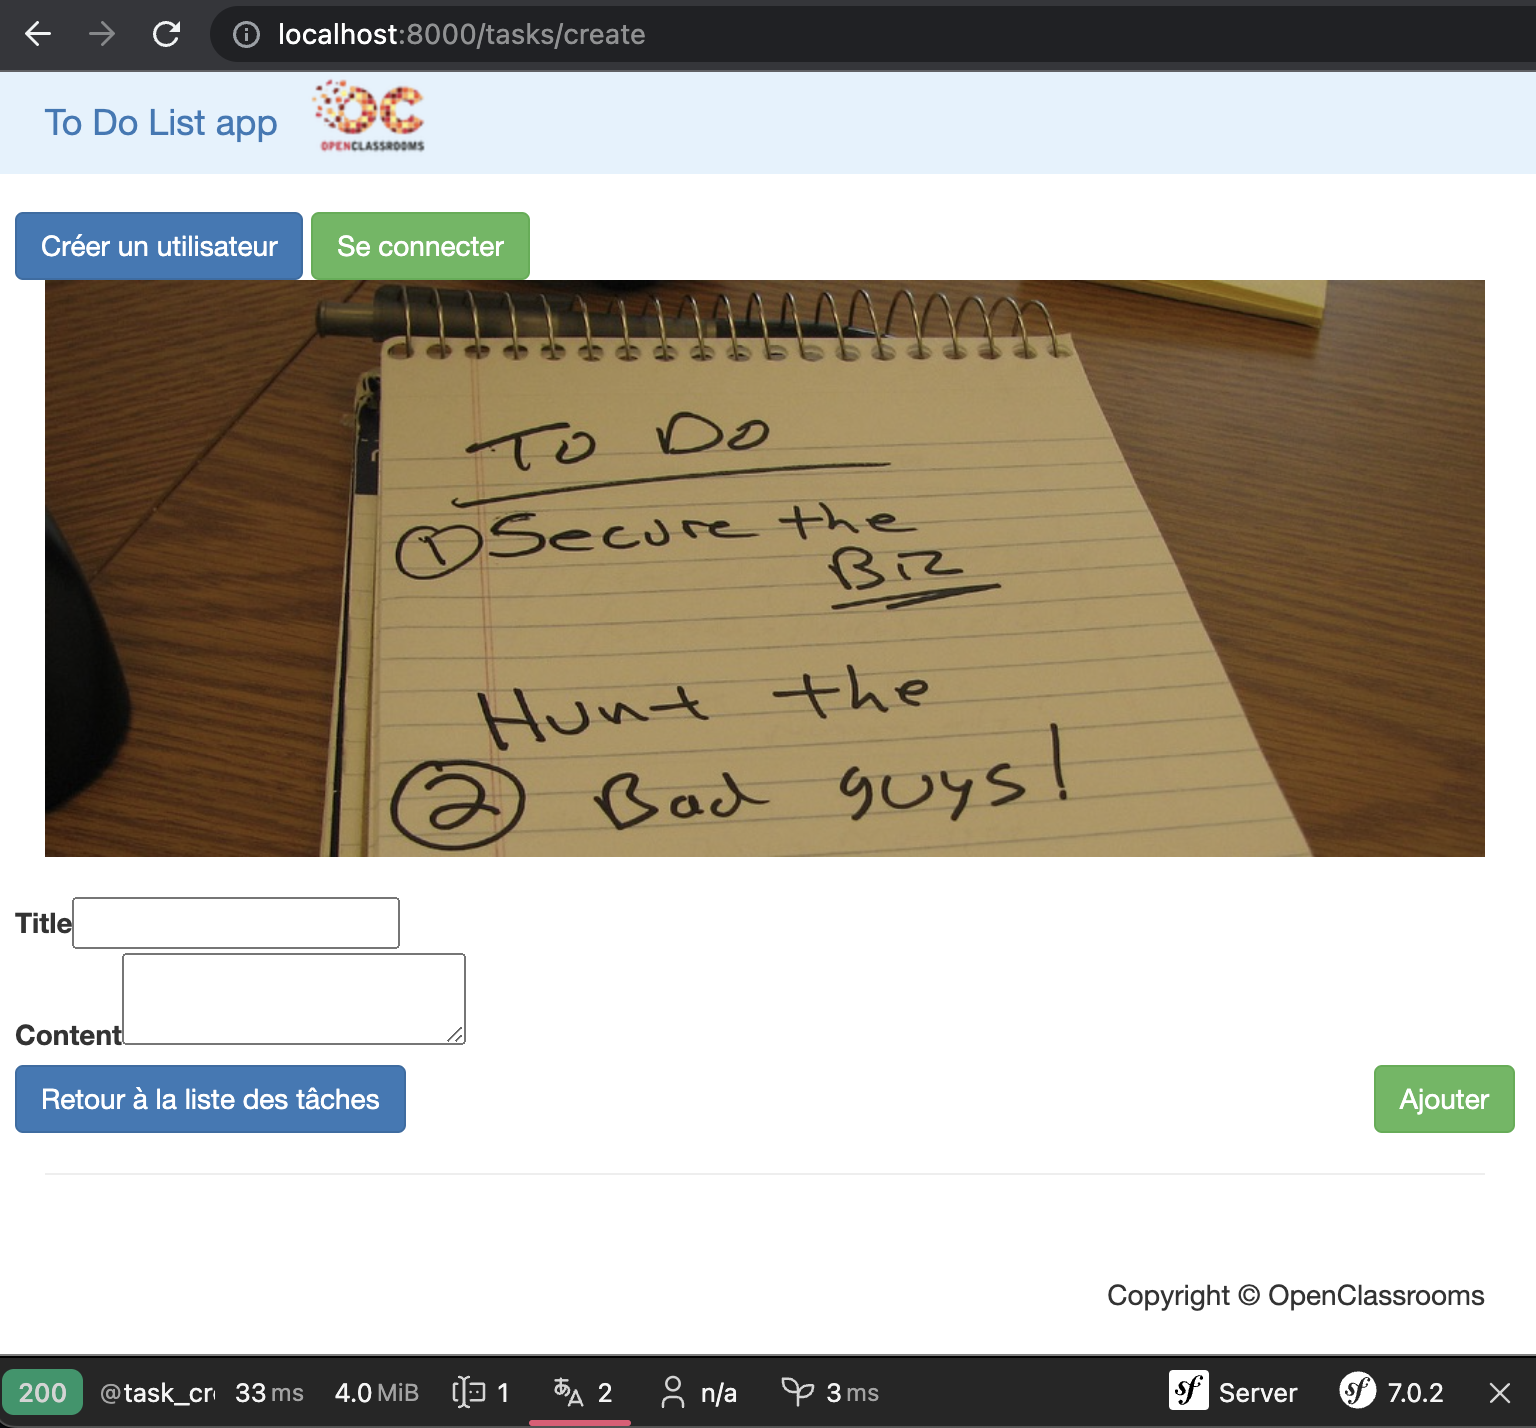
\includegraphics[scale=0.4]{Capture_profiler_avant_modif/Profiler_old_create_task.png}

\subsubsection{Projet avec Symfony 7 après modification}

En utilisant le Profiler de Symfony sur le repository du projet avec Symfony 7 après avoir ajouter les modifications et écrit les tests unitaires et fonctionnels, nous obtenons le résultat suivant : 

\hspace*{2cm}


\includegraphics[scale=0.4]{Capture_profiler_apres_modif/Profiler_new_homepage.png}

\hspace*{2cm}

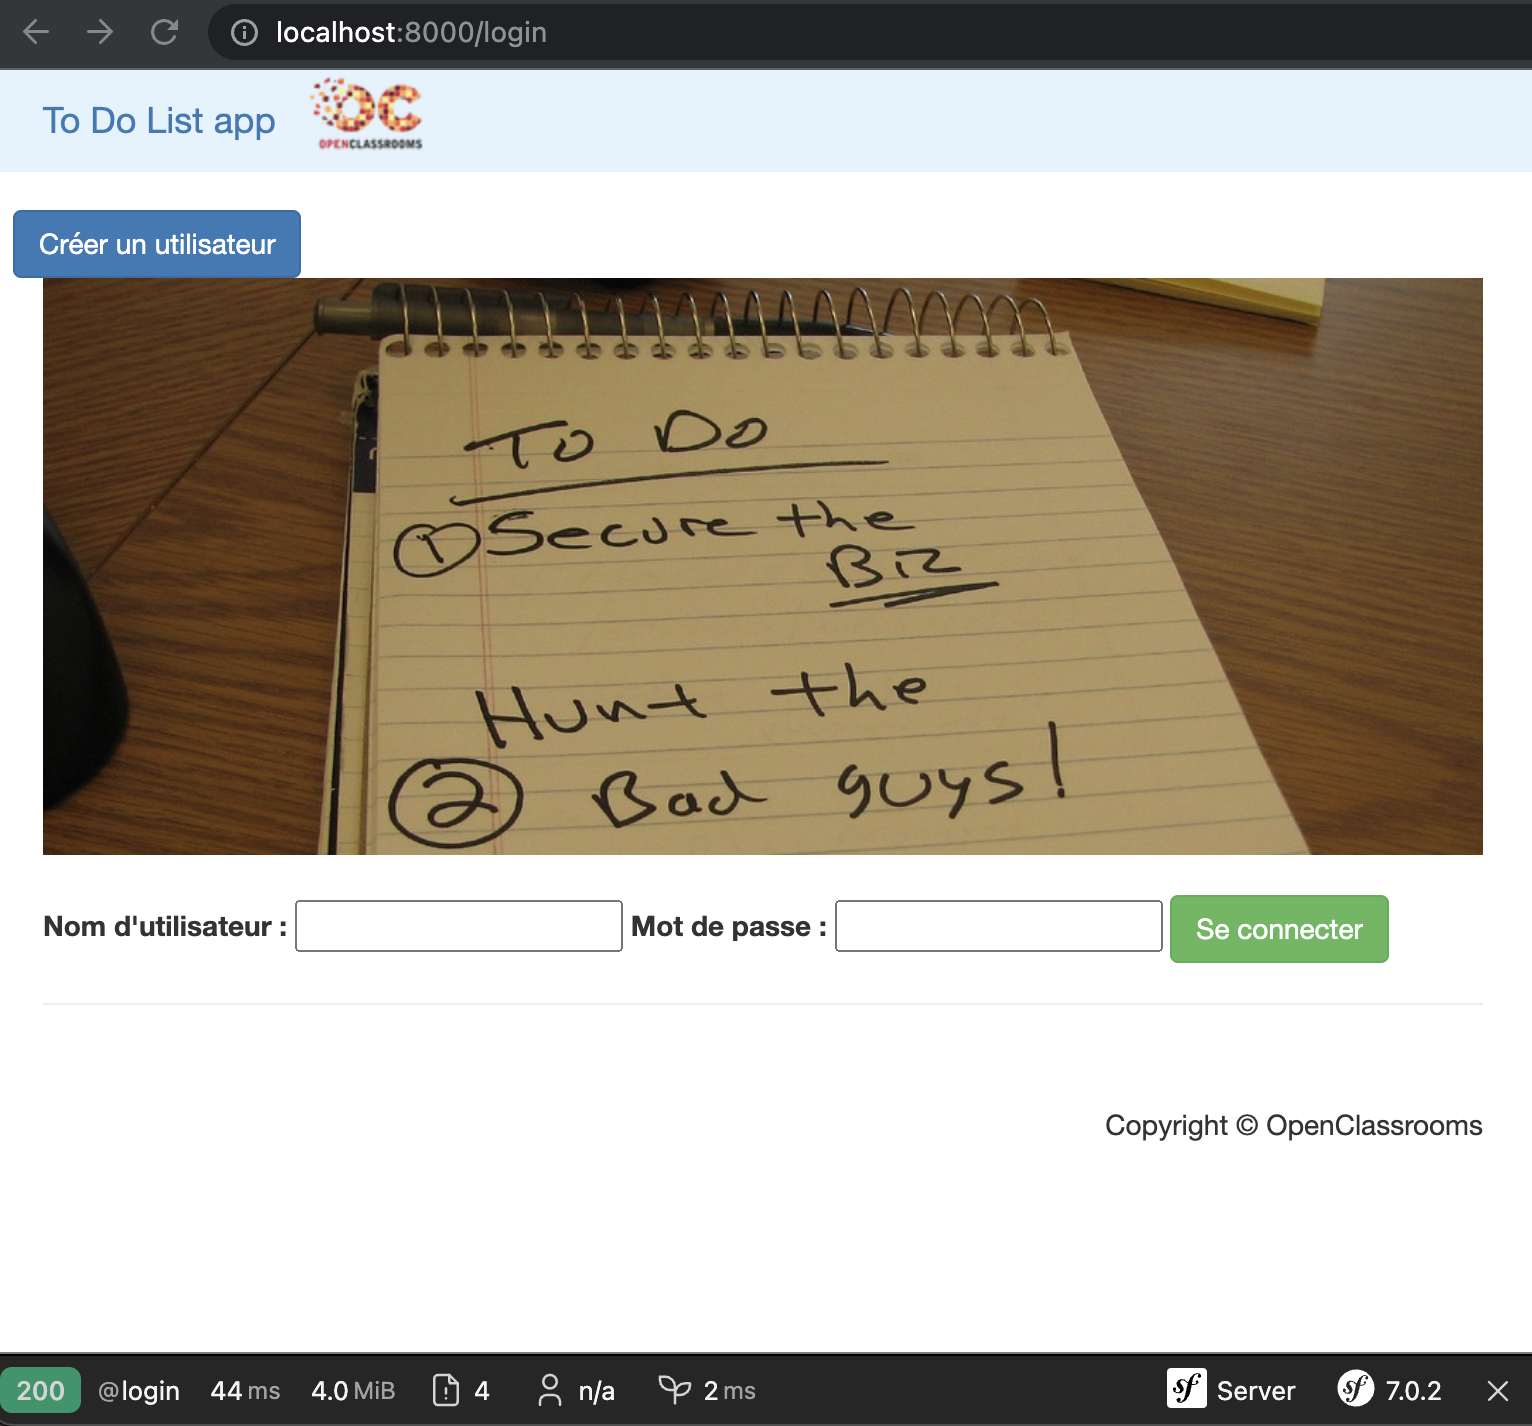
\includegraphics[scale=0.4]{Capture_profiler_apres_modif/Profiler_new_login.png}

\hspace*{2cm}

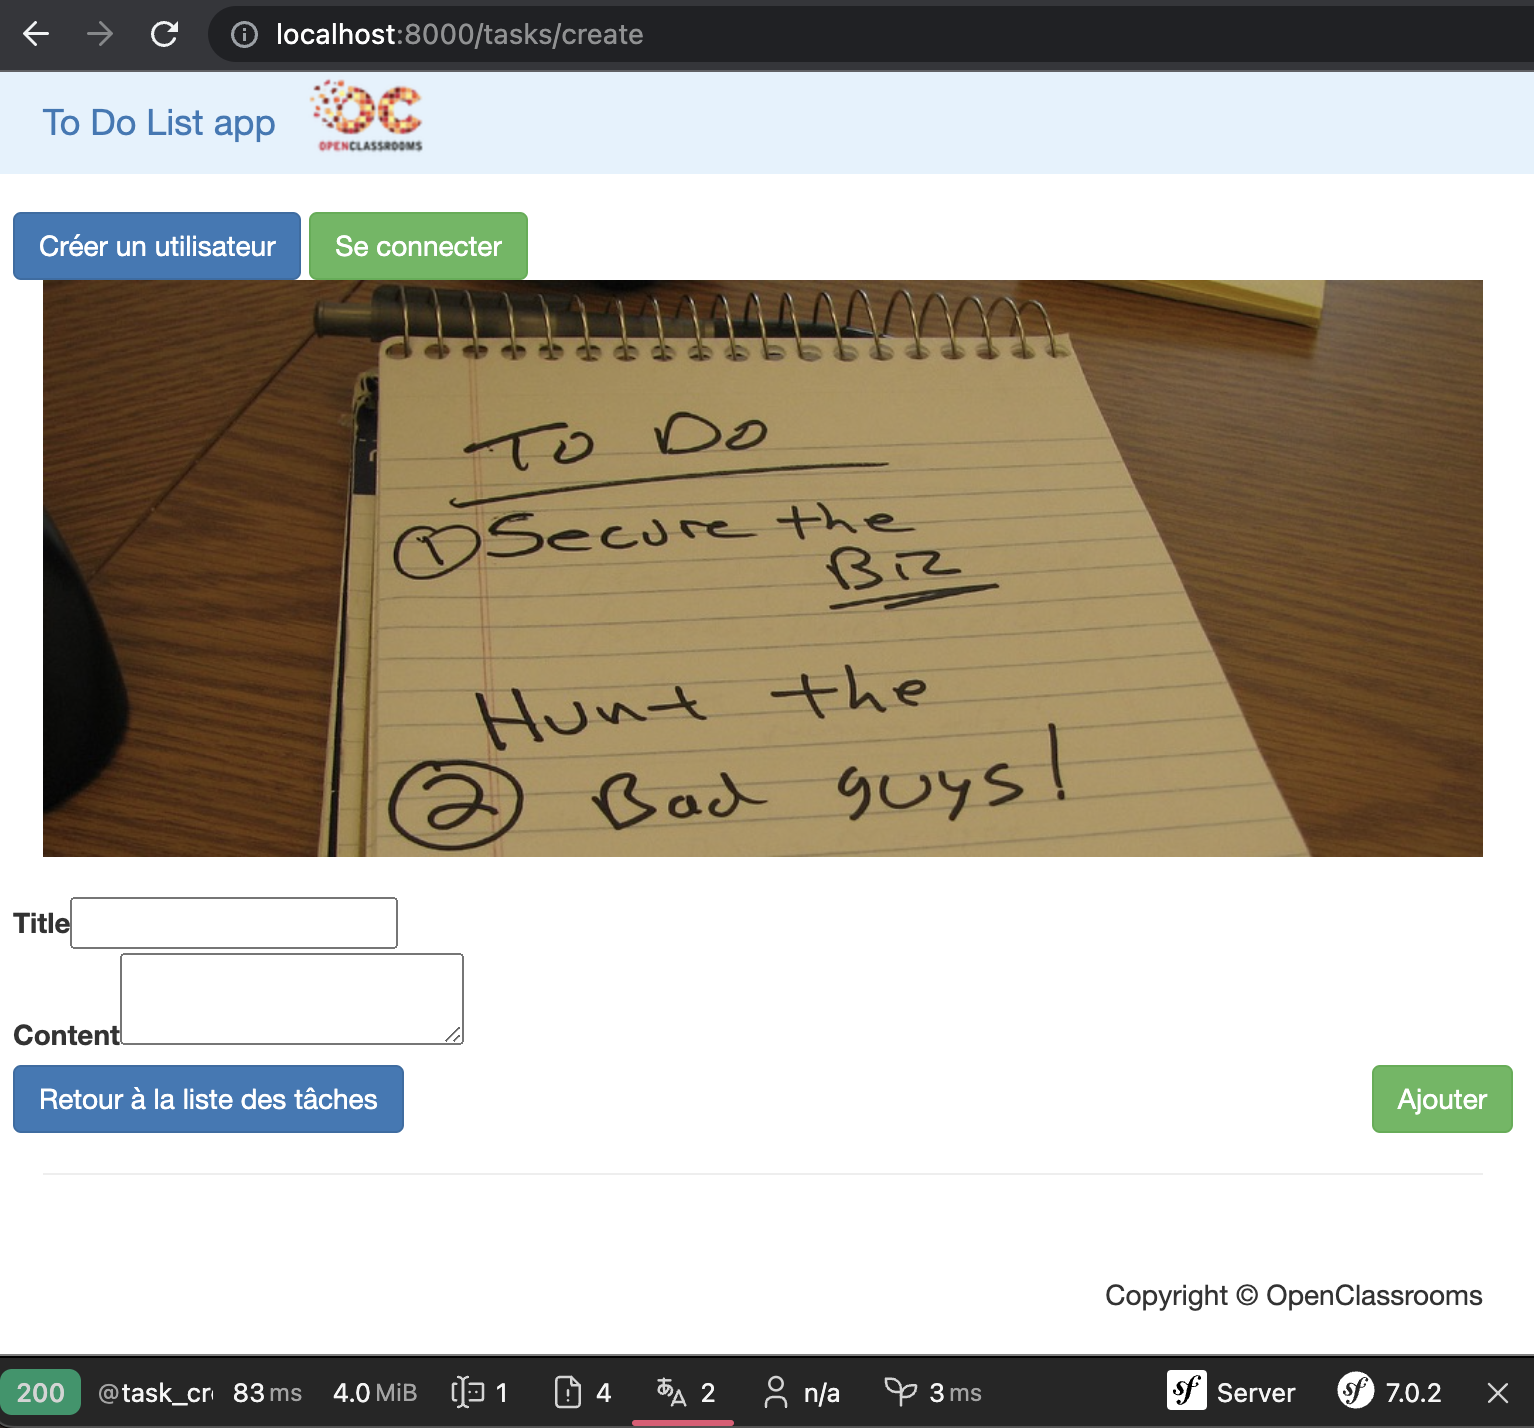
\includegraphics[scale=0.4]{Capture_profiler_apres_modif/Profiler_new_create_task.png}

\subsubsection{Comparaison}

Globalement, le temps de rendu de la page est entre 30 et 85 millisecondes, il peut varier en fonction des performances de la machine mais il reste similaire entre le projet avant modification et après modification.

La consommation de la mémoire a, quand à elle, diminué après modification, sans doute grâce à de l'optimisation de code. 

Le temps de rendu des pages est aussi similaire entre le projet avant modification et le projet après modification. Il est entre 3 et 7 millisecondes pour le projet avant modification et d'environ 2-3 millisecondes pour le projet après modification.











%\subsection{comprendre quel(s) fichier(s) il faut modifier et pourquoi}

%\subsection{comment s’opère l’authentification}

%\subsection{et où sont stockés les utilisateurs}

%\subsection{un document expliquant comment devront procéder tous les développeurs souhaitant apporter des modifications au projet}

%\subsection{le processus de qualité à utiliser ainsi que les règles à respecter}

%\hspace*{2cm}



\newpage
\section*{Conclusion}
\addcontentsline{toc}{section}{Conclusion}

Le projet a été réalisé from scratch pour repartir sur la dernière version de Symfony, puis le code a été copier coller en changeant certaines fonctions pour correspondre à la dernière version de Symfony grâce à la documentation officielle de Symfony. L'audit et la performance ont donc été réalisé avant et après modification sur la dernière version de Symfony.

L'audit et la performance du projet, avant et après modification, est à peu près similaire. Cela est du au fait qu'il n'y a pas beaucoup de modification apportées au projet. 



%Here goes the text.
%\begin{equation}\label{eq:area}
%  S = \pi r^2
%\end{equation}
%One can refer to equations like this: see equation (\ref{eq:area}). One can also
%refer to sections in the same way: see section \ref{sec:nothing}. Or
%to the bibliography like this: \cite{Cd94}.

%\subsection{Subsection}\label{sec:nothing}

%More text.

%\subsubsection{Subsubsection}\label{sec:nothing2}

%More text.

% Bibliography
%-----------------------------------------------------------------
%\begin{thebibliography}{99}

%\bibitem{Cd94} Author, \emph{Title}, Journal/Editor, (year)

%\end{thebibliography}

\end{document}
